\documentclass{article}

\usepackage[utf8]{inputenc}
\usepackage[T1]{fontenc}
\usepackage{lipsum}
\usepackage{graphicx}
\usepackage{amsmath}
\usepackage[margin=1in]{geometry}
\usepackage{titlesec}

\titleformat{\section}
{\LARGE\bfseries}{\thesection}{1em}{}

\titleformat{\subsection}
{\Large\bfseries}{\thesection}{1em}{}

\begin{document}

\pagestyle{empty}

\section*{Diagramma delle interazioni pag. 205}
\large
I diagrammi comportamentali sono i più comuni diagrammi di interazione. Si concentrano sullo scambio di messaggi tra diverse lifelines.\\
I diagrammi comportamentali descrivono le interazioni concentrandosi sulla sequenza di messaggi che vengono scambiati e i loro eventi specifici corrispondenti.
\begin{center}
    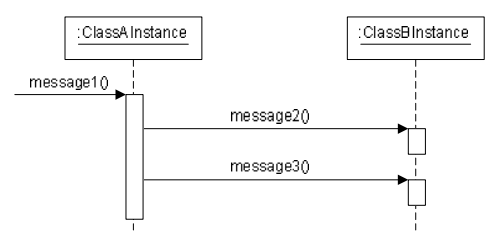
\includegraphics[width=0.5\textwidth]{foto 2.png}
\end{center}
\textit{Spiegazione}: le interazioni avvengono sotto forma di scambi di messaggi con un verso. Questo schema viene utilizzato per analisi(interazioni tra attori-sistema in un caso d'uso) e per design. Le linee tratteggiate vengono definite \textbf{lifeline}, mentre le freccie direzionate indicano dei messaggi (come Insert coin e Update credit). \textbf{:VendingMachine} è una istanza di VendingMachine, mentre \textbf{loop} e \textbf{opt} sono situazioni ripetibili più volte o opzionali.\\
Vediamo ora gli elementi di un diagramma comportamentale:
\begin{center}
    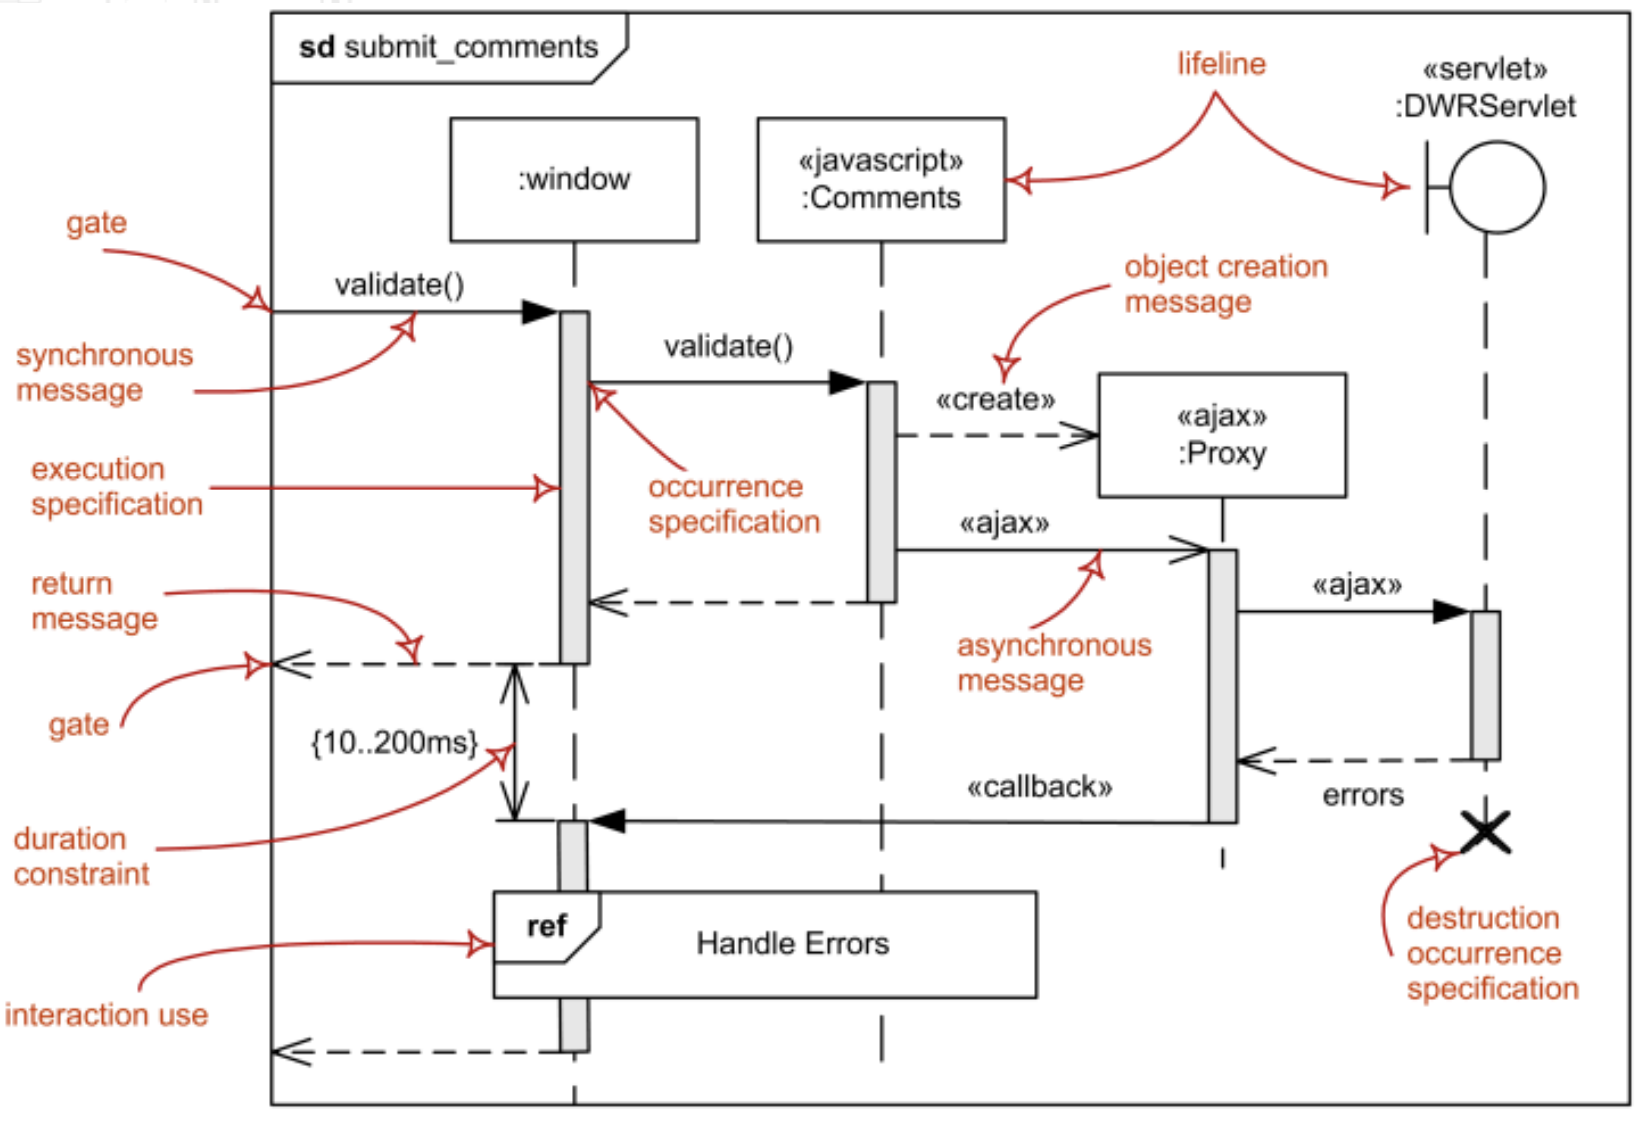
\includegraphics[width=1\textwidth]{foto 3.png}
\end{center}
\textit{Nota Bene}: se non sono presenti \textit{gate} l'utilizzo del rettangolo esterno è opzionale.\\
\textit{Occurrence specification}: quando arriva o viene mandato un messaggio.

\subsection*{Lifeline}
\large

Una \textbf{lifeline} è un elemento che rappresenta un partecipante individuale nella interazione. Mentre le parti e le caratteristiche strutturali possono avere moltiplicità maggiore di 1, le lifelines rappresentano soltanto una entità che interagisce.
\begin{center}
    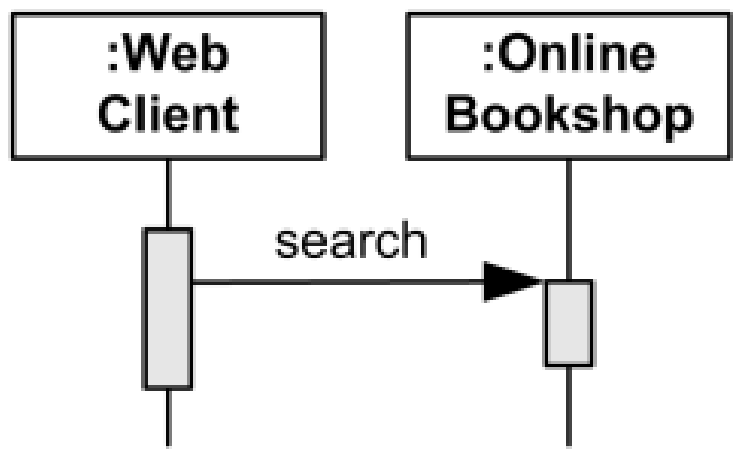
\includegraphics[width=0.6\textwidth]{foto 4.png}
\end{center}

\subsection*{Messaggi}
\large

Un \textbf{messaggio} è un elemento che definisce uno specifico tipo di comunicazione tra le diverse lifelines di una interazione. Il messaggio specifica non solo il tipo di comunicazione, ma anche il mittente ed il destinatario. Mittente e destinatario di solito sono due occorrenze specifiche (endpoint del messaggio).\\
Un messaggio può rappresentare una chiamata ad operazione e l'inizio della sua esecuzione o l'invio e la ricezione di un segnale. In base al tipo di azione utilizzata per generare il messaggio, il messaggio può essere:
\begin{enumerate}
    \renewcommand{\labelenumi}{-}
    \item Chiamata syncrona/asyncrona
    \item Segnale asyncrono
    \item Risposta
    \item Creare 
    \item Cancellare
\end{enumerate}
\textit{Chiamata syncrona}\\
Una \textbf{chiamata syncrona} rappresenta solitamnte una chiamta ad operazione; viene mandato un messaggio e sospesa l'esecuzione fino all'arrivo di una risposta. Le chiamate a messaggio syncrone vengono rappresentate graficamente con una freccia con punta colorata. 
\begin{center}
    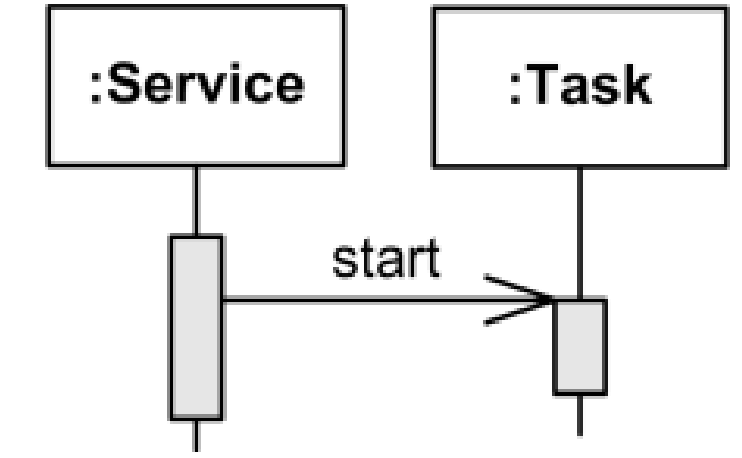
\includegraphics[width=0.4\textwidth]{foto 5.png}\\
\end{center}
\textit{Chiamata asyncrona}\\
Una \textbf{chiamata asyncrona} rappresenta solitamnte una chiamta ad operazione; viene mandato un messaggio e si procede con l'esecuzione senza aspettare l'arrivo di una risposta. Le chiamate a messaggio asyncrone vengono rappresentate graficamente con una freccia con punta aperta. 
\begin{center}
    
\includegraphics[width=0.4\textwidth]{foto 6.png}\\
\end{center}
\textit{Risposta}\\
Una \textbf{risposta} ad una chiamata ad operazione vengono rappresentate graficamente con una freccia tratteggiata con punta aperta (simile al messaggio di creazione).
\begin{center}
    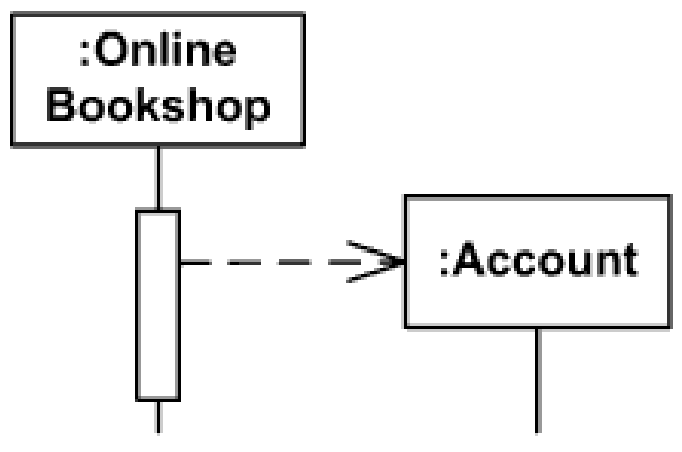
\includegraphics[width=0.4\textwidth]{foto 7.png}\\
\end{center}
\textit{Creare}\\
Un messaggio di \textbf{creazione} viene inviato ad una lifeline per crearsi. E' pratica comune inviare un messaggio di creazione ad un oggetto ancora non esistente per crearsi.
\begin{center}
    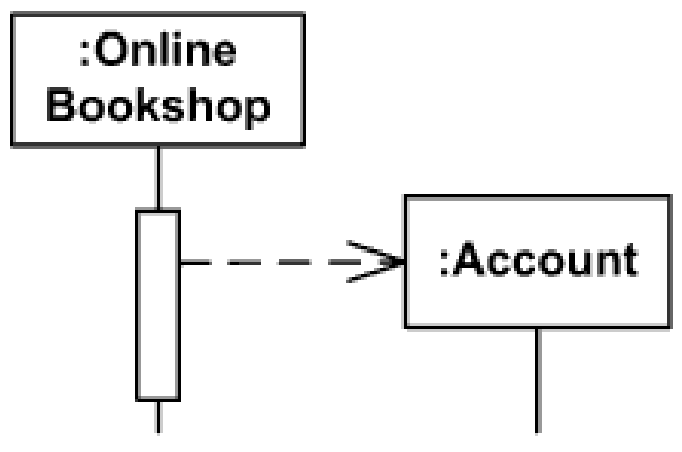
\includegraphics[width=0.4\textwidth]{foto 8.png}\\
\end{center}
\textit{Cancellare}\\
Un messaggio di \textbf{cancellazione} viene inviato ad una lifeline per terminarla. La lifeline di solito termina con una croce nella forma di una X che denota la distruzione dell'evento.
\begin{center}
    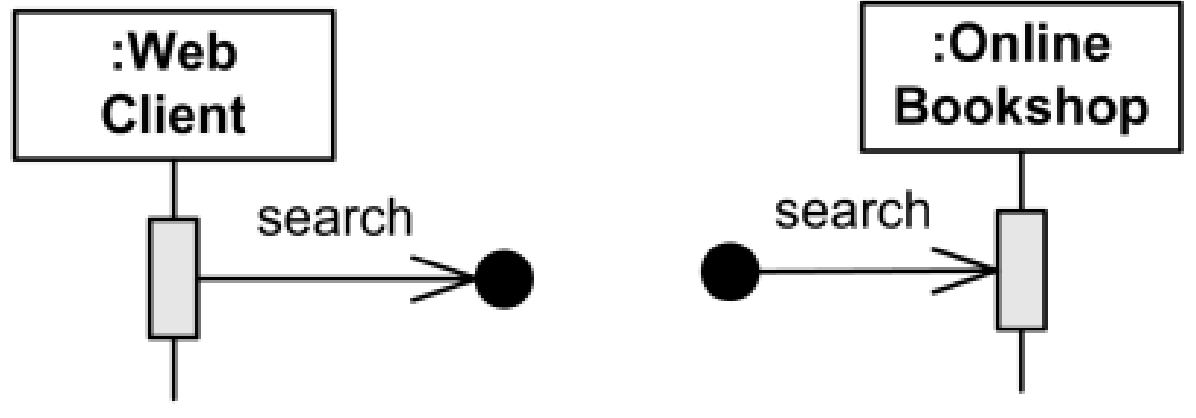
\includegraphics[width=0.4\textwidth]{foto 9.png}\\
\end{center}

\subsection*{Lost \& founds}
\large
\begin{center}
    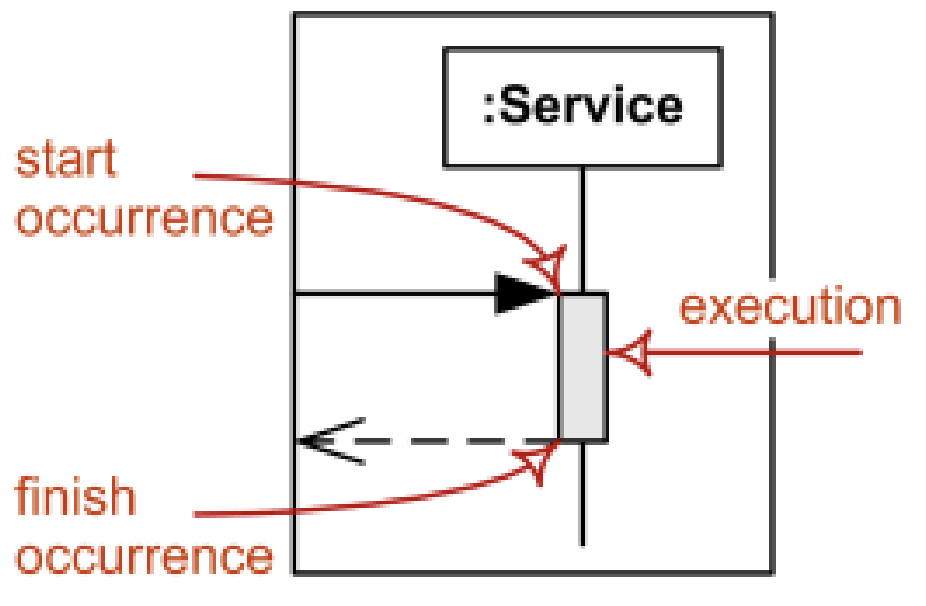
\includegraphics[width=0.4\textwidth]{foto 10.png}\\
\end{center}
Non so davvero cosa scrivere qui, aiuto!

\subsection*{Gate}
\large

Un \textbf{gate} è la fine di un messaggio, un punto di connessione che unisce un messaggio esterno al frammento di interazione con uno interno al frammento di interazione.
\begin{center}
    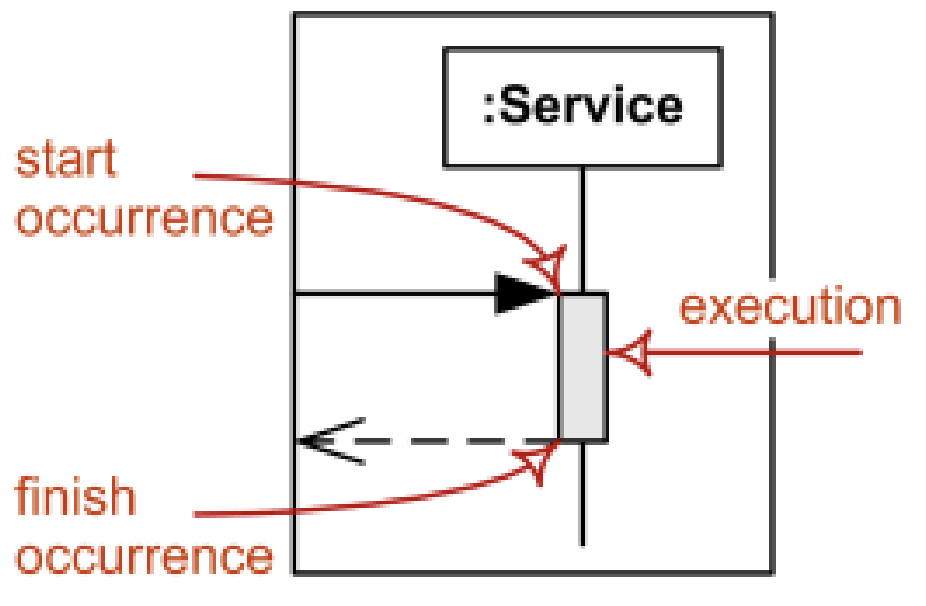
\includegraphics[width=0.4\textwidth]{foto 11.png}\\
\end{center}

\subsection*{Frammento di interazione}
\large

Un \textbf{frammento di interazione} è un elemento che rappresenta la più generale unità di interazione. Ogni frammento di interazione è concettualmente come un interazione. Non c'è una notazione generale per i frammenti di interazione. Le sue sottoclassi definiscono le proprie notazioni. Alcuni esempi di frammenti di interazione sono le \textit{occorrenze}, le \textit{esecuzioni}, lo \textit{stato invariato}, i \textit{frammenti combinati} e le \textit{interazioni d'uso}.

\subsection*{Occorrenza}
\large

Una \textbf{occorrenza} (\textbf{specifica di occorrenza}) è un frammenti di interazione che rappresenta un momento preciso nel tempo (evento) all'inzio o alla fine di un messaggio o all'inizio o alla fine di un'esecuzione.\\
Una specifica di occorrenza è una delle unità semantiche di interazione di base. Il significato di queste interazioni è specificato dalle sequenze di occorrenze descritte dalle specifiche di occorrenza.

\subsection*{Esecuzione}
\large

Una \textbf{esecuzione} (\textbf{specifica di esecuzione, informalmente chiamata attivazione}) è un frammento di interazione che rappresenta un periodo nel ciclo di vita del partecipante nel quale:
\begin{enumerate}
    \renewcommand{\labelenumi}{-}
    \item esegue un'azione o comportamento nel suo ciclo di vita
    \item manda un segnale ad un altro partecipante
    \item aspetta una risposta da un altro partecipante
\end{enumerate}
\begin{center}
    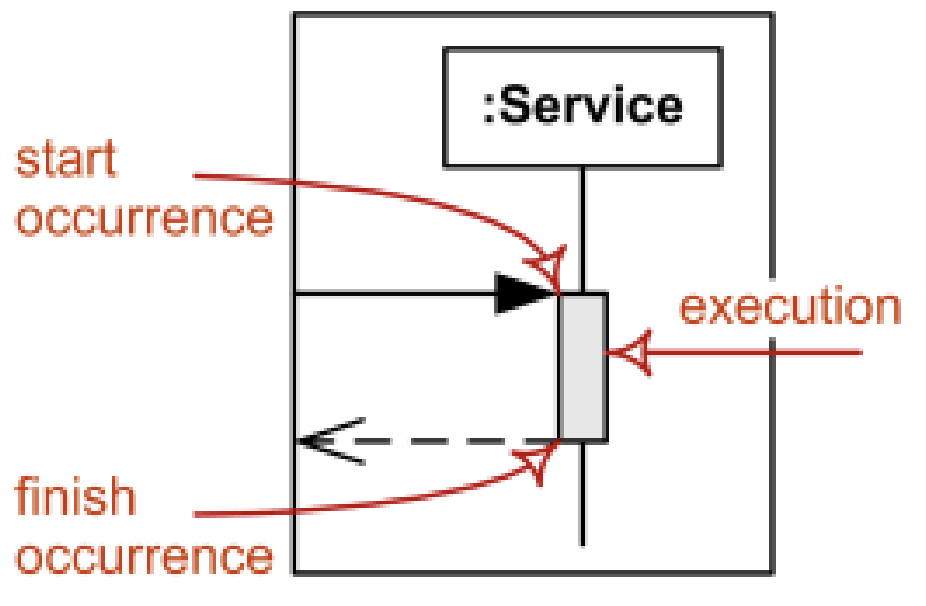
\includegraphics[width=0.4\textwidth]{foto 12.png}\\
\end{center}

\subsection*{Combinazione di frammenti}
\large

Una \textbf{combinazione di frammenti} è un frammento di interazione che definisce una combinazione di frammenti di interazione. Viene definito da un operatore di interazione e dai suoi operatori. Tramite l'uso di combinazioni di frammenti l'utente è in grado di descrivere un numero di tracce maggiore in un modo più compatto e conciso. Le combinazioni di frammenti possono avere anche vincoli di interazione (guardie). Alcuni operatori possono essere:
\begin{enumerate}
    \renewcommand{\labelenumi}{-}
    \item \textbf{alt}: alternative
    \item \textbf{opt}: opzionale
    \item \textbf{loop}: iterazione 
    \item \textbf{break}
    \item \textbf{par}: parallelo
    \item \textbf{strict}: sequenza vincolante
    \item \textbf{seq}: sequenza debole
    \item \textbf{critical}: regione critica 
    \item \textbf{ignore}: ignorare
    \item \textbf{consider}: considerazione
    \item \textbf{assert}: affermazione
    \item \textbf{neg}: negativo
\end{enumerate}
\begin{center}
    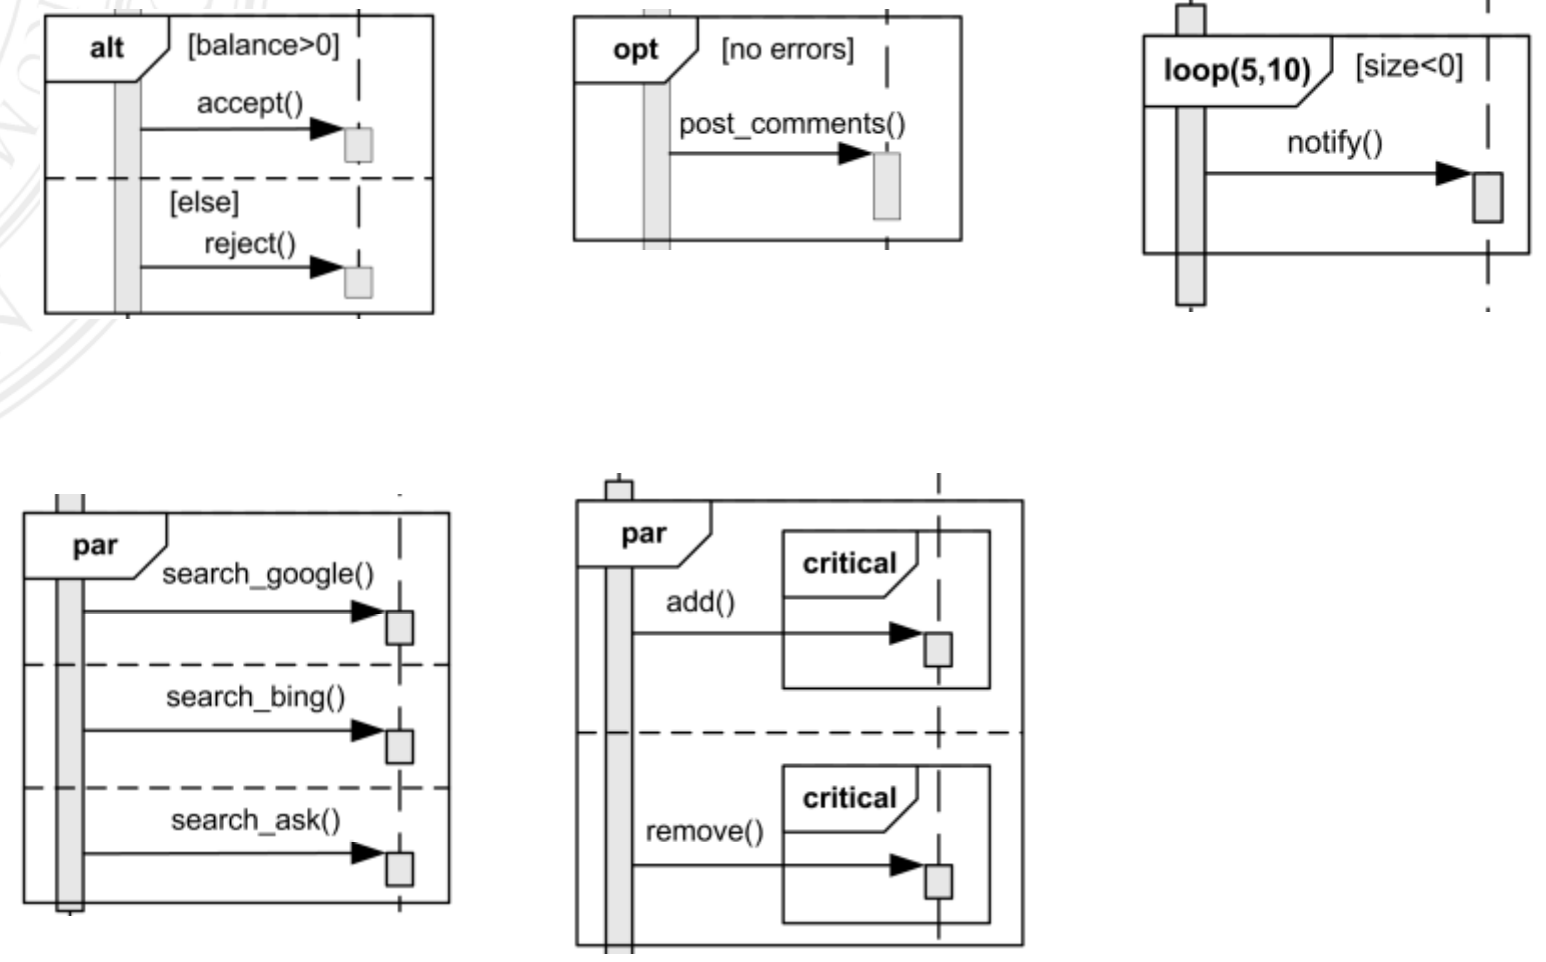
\includegraphics[width=0.8\textwidth]{foto 13.png}
\end{center}
spiegare questa foto!!!

\subsection*{Interazione d'uso}
\large

Un \textbf{interazione d'uso} è un frammento di interazione che permette di usare (o chiamare) un altra interazione. Grandi e complessi diagrammi comportamentali possono essere semplificati con interazioni d'uso. E' anche solito riutilizzare alcune interazioni tra molte altre interazioni.
\begin{center}
    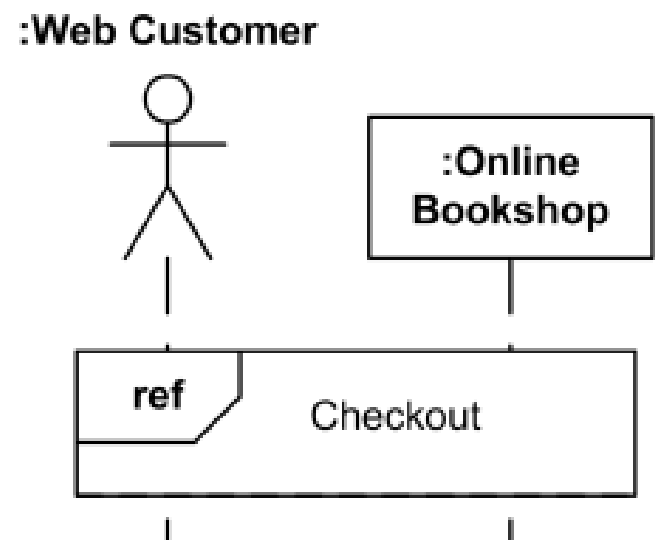
\includegraphics[width=0.4\textwidth]{foto 14.png}
\end{center}

\subsection*{Linee guida per i  diagrammi comportamentali}
\large

Non generalizzare troppo i comportamenti. Quando vengono utilizzati i diagrammi comportamentali per analisi:
\begin{enumerate}
    \renewcommand{\labelenumi}{-}
    \item un caso d'uso può essere descritto da più di un diagramma comportamentale
    \item il tipo di azione del messaggio può essere deciso nel momento del design
    \item nessun messaggio tra lifelines che appartengono a elementi del sistema
\end{enumerate}

\subsection*{Diagrammi di comunicazione}
\large

Un \textbf{diagramma di comunicazione} mostra le interazioni tra diverse lifeline usando una forma non prestabilita. Possono essere convertiti in diagrammi comportamenti (ma non viceversa in UML 2). Viene assunto che i messaggi vengono ricevuti nello stesso ordine nel quale vengono generati. Vengono quindi numerati per garantire il loro ordine corretto. Un diagramma di comunicazione può contenere frames, lifelines e messaggi.
\begin{center}
    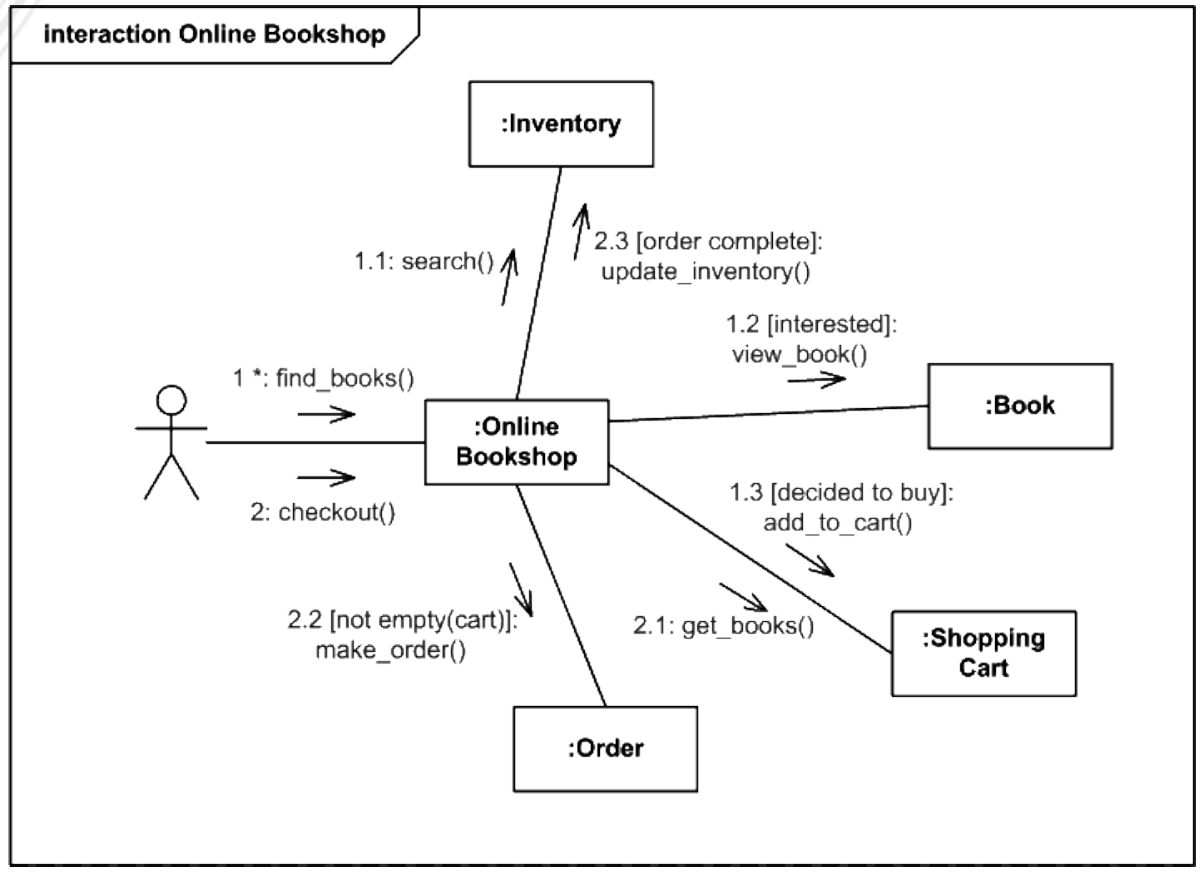
\includegraphics[width=0.7\textwidth]{foto 15.png}
\end{center}
spiegare questa foto!!!\vspace{14pt}\\
La notazione per i messaggi nei diagrammi di comunicazione segue le stesse regole usate nei diagrammi comportamentali. In modo da capire la dinamica evolutiva del sistema, i messaggi hanno una sequenza di espressione.
ste ultime due slide non le ho capite per nulla!!!

\end{document}